\subsection{Convertidor CC-CC Conmutado}

Un convertidor CC-CC es un dispositivo electrónico que tiene como objetivo convertir una tensión continua, generalmente no regulada (es decir que no es fija), $V_{in}$ a la entrada, a una tensión continua regulada $V_{out}$ de distinta magnitud a la salida, transfiriendo la mayor cantidad de energía posible de la entrada hacia la salida. Dependiendo del tipo de convertidor, esta tensión de salida puede ser menor, mayor o tanto menor como mayor a la tensión de entrada.\\

Estos convertidores son de interés para nuestra aplicación, ya que la tensión $V_{stack}$ que entrega la pila (ecuación \ref{v_stack}) es una tensión continua no regulada, que varía apreciablemente con la corriente demandada; mientras que a la salida se demanda una tensión fija y regulada $V_{bus}$ para conectar al bus de continua del sistema híbrido de la figura \ref{SHGE}.\\

La forma más básica que se podría concebir para un dispositivo que cumpla esta función es la de un simple divisor resistivo, en el cual la tensión $V_{out}$ depende de las resistencias $R_1$ y $R_2$ y la tensión de entrada $V_{in}$.

\begin{equation*}
    V_{out} = V_{in}\cdot\frac{R_2}{R_1+R_2}
\end{equation*}

Entonces, variando la relación entre $R_1$ y $R_2$, se puede variar la tensión $V_{out}$ entre tensión nula y $V_{in}$. Sin embargo, se necesita solo un análisis superficial de esta topología para ver que no es viable para ningún tipo de aplicación, más que nada por su pobre eficiencia energética (para obtener una tensión igual a la mitad de la entrada, se pierde la mitad de la potencia en disipación resistiva).\\

Los convertidores CC-CC se suelen separar en dos principales categorías: los {\Medium reguladores lineales}, que son un caso complejizado del divisor resistivo donde se utiliza un transistor como resistencia variable (además de un diodo para regular la tensión de salida); y los {\Medium convertidores conmutados}, en los cuales uno o más transistores, actuando como llaves, son conmutados a alta frecuencia y junto con dispositivos que almacenan energía (como inductores y capacitores) producen una tensión continua a la salida.\\

Dado que para esta plataforma se utiliza un convertidor conmutado (principalmente por su gran ventaja en eficiencia energética), se enfocará el análisis únicamente en éstos; comenzando por una explicación de los conceptos básicos necesarios para comprender su funcionamiento.\\

\subsubsection{Conceptos Básicos de Convertidores CC-CC Conmutados}

Como se detalló más arriba, los convertidores CC-CC conmutados consisten, en su forma más básica, en una fuente de continua no regulada a la entrada; y un transistor (que puede ser BJT, MOSFET o IGBT) que, mediante una excitación en su tercer terminal, se conmuta entre los modos de alta impedancia e impedancia nula, actuando como llave abierta y llave cerrada respectivamente. La proporción del tiempo total de ciclo ($T_s$) en la que el transistor está conduciendo ($t_{on}$) se denomina {\Medium ciclo de trabajo} o {\Medium \textit{duty cycle}} y se suele simbolizar con la {\Medium letra \textit{D}}. Como se verá más adelante, este es un parámetro crucial para el funcionamiento de este tipo de convertidores, ya que controlándolo se puede variar el nivel de tensión y corriente de salida.

\begin{figure}[H]
    \centering
    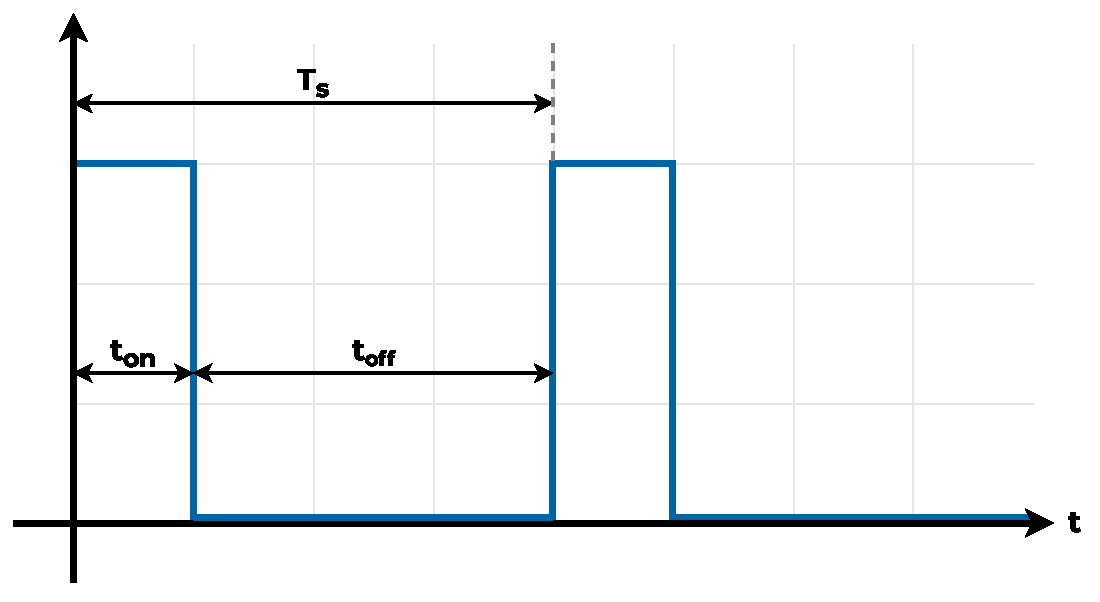
\includegraphics[scale=0.5]{Imagenes/Duty Cycle.pdf}
    \caption{Una forma de onda cuadrada con ciclo de trabajo $D$ del 25 \%.}
    \label{dutycycle}
\end{figure}

Los convertidores CC-CC conmutados se clasifican en dos grandes grupos, usando como criterio la existencia de aislación galvánica entre la entrada no regulada y la salida regulada:

\begin{itemize}
    \item {\SemiBold Convertidores No Aislados:} son los convertidores que no tienen aislación galvánica entre entrada y salida, como por ejemplo los convertidores reductores y elevadores (\textit{buck} y \textit{boost}), y por lo tanto son los mas simples de los dos tipos.
    \item {\SemiBold Convertidores Aislados:} son los convertidores que tienen su entrada y salida aisladas galvánicamente por medio de un transformador de alta frecuencia, por ejemplo los de tipo \textit{flyback} y \textit{forward}. El convertidor de esta plataforma, de tipo puente completo, cae dentro de esta categoría.
\end{itemize}

En la siguiente sección se va a detallar el funcionamiento de los dos convertidores no aislados más sencillos, los convertidores reductor y elevador, a manera de introducir los principios de funcionamiento de convertidores conmutados que van a ser necesarios para luego poder entender las topologías más complejas que se utilizan en esta plataforma.\\

\subsubsection{Ejemplo Básico de un Convertidor CC-CC Conmutado}

La forma más básica posible de un convertidor conmutado tiene un esquema circuital similar al convertidor lineal mencionado más arriba, con la diferencia de que el transistor, (que previamente actuaba como una resistencia variable para conformar el divisor resistivo) en este caso, actúa como el interruptor del circuito, conmutando entre llave abierta y cerrada (figura \ref{proto_reductor}). Para este análisis vamos a considerar que el dispositivo semiconductor actúa como una llave ideal, sin impedancia cuando está cerrado y con impedancia infinita cuando está abierto.

\begin{figure}[H]
    \centering
    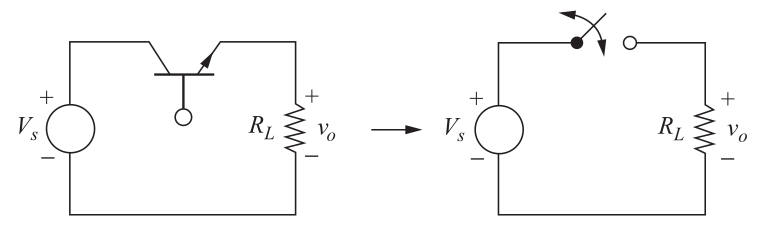
\includegraphics[scale=0.4]{Imagenes/Proto Reductor.png}
    \caption{Circuito de un convertidor conmutado básico, con el transistor $Q_1$ actuando como llave (Placeholder).}
    \label{proto_reductor}
\end{figure}

Entonces, si se aplica una señal de control como la de la figura \ref{dutycycle} al interruptor, durante un período $T_s$ de la señal ocurren dos cosas distintas:

\begin{itemize}
    \item {\SemiBold Durante el tiempo $\mathbf{t_{on}}$}, el transistor se comporta como una llave cerrada y permite la libre circulación de corriente. Entonces, esta corriente circula por la carga $R_L$, donde, por la Ley de Ohm, cae una tensión igual a la tensión de entrada, es decir, que la tensión de salida {\Medium \textit{v\textsubscript{o}} es igual a la tensión de entrada \textit{V\textsubscript{s}}}.
    \item {\SemiBold Durante el tiempo $\mathbf{t_{off}}$}, el transistor pasa a comportarse como una llave abierta, por lo que restringe completamente la circulación de corriente. Por lo tanto, la caída de tensión en la carga $R_L$ es nula, es decir, que la tensión de salida {\Medium \textit{v\textsubscript{o}} es nula}.
\end{itemize}

Uniendo estos dos comportamientos, se puede ver que la forma de la tensión de salida es análoga a la forma de onda cuadrada que controla al interruptor (de la figura \ref{dutycycle}), oscilando entre \SI{0}{\volt} y $V_s$.

\begin{equation}\label{valor_medio_reductor}
    \bar{v}_o = \frac{1}{T_s}\int\limits^{T_s}_0 v_0(t) dt = \frac{1}{T_s}\int\limits^{DT_s}_0 V_s dt = V_s\cdot D \leq V_s
\end{equation}

Calculando el valor medio de $v_o$ en la ecuación \ref{valor_medio_reductor}, este resulta ser directamente proporcional al ciclo de trabajo de la señal de control, variando entre \SI[]{0}[]{\volt} y la tensión de entrada $V_s$, para ciclos de trabajo entre \num{0} y \num{1} respectivamente. Es decir, la {\Medium tensión media de salida es menor o igual a la de entrada} (esto se puede ver sin necesidad de cálculo, ya que si la salida es igual a la entrada por una proporción del tiempo total, su valor medio necesariamente debe ser menor, o como mucho igual, al valor de la entrada) y se controla directamente con la variación de $D$.\\

En principio, si se considera el transistor como interruptor ideal, la eficiencia de este dispositivo es del 100 \%, ya que durante el tiempo $t_{off}$ no circula ninguna corriente (por lo tanto no hay disipación de ningún tipo), y durante $t_{on}$ no hay caída de tensión en el transistor. En la realidad, los transistores no actúan como llaves ideales, si no que tienen ciertas no idealidades que resultan en pérdidas de energía: no tienen impedancia perfectamente nula como llave cerrada, ni impedancia infinita como llave abierta, además de poseer pérdidas a la hora de conmutar.\\

Sin embargo, en muchos casos y aplicaciones (incluido el de este trabajo) no es suficiente obtener una salida de pulsos y controlar su tensión media, si no que se necesita obtener una tensión puramente continua directamente en la salida, como puede ser el caso para una fuente de alimentación.\\

Para solucionar este problema, se agrega un filtro pasa-bajos LC a la salida luego del interruptor, que se encarga de eliminar los componentes de alta frecuencia relacionados a la conmutación, dejando pasar únicamente los componentes de continua. El convertidor que resulta es la topología de convertidor CC-CC conmutado más sencilla: el {\Medium convertidor reductor} o {\Medium \textit{buck}} de la figura \ref{reductor}.

\begin{figure}[H]
    \centering
    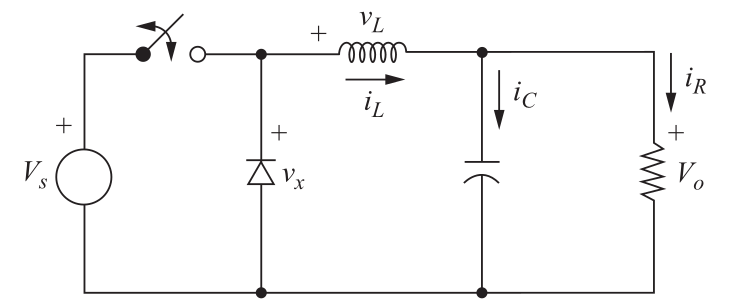
\includegraphics[scale=0.4]{Imagenes/Reductor.png}
    \caption{Circuito de un convertidor reductor o buck completo (Placeholder).}
    \label{reductor}
\end{figure}

Además del filtro ya mencionado, se agrega un diodo de rueda libre o \textit{flyback} en derivación entre el transistor y el inductor (diodo $D_1$ de la figura \ref{reductor}). Este dispositivo cumple la función de proveer un camino de circulación para la corriente $i_L$ del inductor cuando el interruptor se encuentra abierto, que resulta necesario ya que la corriente sobre un inductor no puede variar abruptamente. Entonces, cuando el interruptor está abierto, el diodo entra en polarización directa y permite la circulación de corriente; mientras que cuando está el interruptor cerrado, el diodo se polariza con una tensión inversa $V_s$ y actúa como un circuito abierto, eliminando su influencia sobre el convertidor durante $t_{on}$.\\



\begin{center}
    {\Thin Thin} {\ExtraLight ExtraLight} {\Light Light} Regular {\Medium Medium}  {\SemiBold SemiBold} {\Bold Bold} {\ExtraBold ExtraBold} {\Black Black}
\end{center}